\documentclass[aspectratio=169, 10pt]{beamer}

% --- PACKAGES ---
\usepackage[utf8]{inputenc}
\usepackage{tikz}
\usetikzlibrary{shapes.geometric, arrows.meta, positioning, fit, backgrounds}
\usepackage{booktabs}
\usepackage{array}
\usepackage{xcolor}

% --- COLOR PALETTE ---
\definecolor{NavyBg}{HTML}{0A2540}
\definecolor{CardBg}{HTML}{0F3358}
\definecolor{AmberAccent}{HTML}{FF8A3D}
\definecolor{TealAccent}{HTML}{6BE6C1}
\definecolor{TextInk}{HTML}{DCE8F5}
\definecolor{TextDim}{HTML}{8FA9C4}

% --- BEAMER THEME CUSTOMIZATION ---
\setbeamercolor{background canvas}{bg=NavyBg}
\setbeamercolor{normal text}{fg=TextInk}
\setbeamercolor{frametitle}{bg=CardBg, fg=white}
\setbeamercolor{title}{fg=white}
\setbeamercolor{subtitle}{fg=AmberAccent}
\setbeamercolor{item}{fg=TealAccent}
\setbeamercolor{subitem}{fg=AmberAccent}
\setbeamercolor{block title}{bg=CardBg, fg=AmberAccent}
\setbeamercolor{block body}{bg=CardBg!50!NavyBg, fg=TextInk}

\setbeamertemplate{navigation symbols}{}
\setbeamertemplate{footline}{%
  \hfill\raisebox{6pt}{\color{TextDim}\scriptsize\textrm{\insertframenumber\,/\,\inserttotalframenumber}}\hspace{8pt}
}
\setbeamertemplate{itemize items}[circle]
\setlength{\parskip}{0pt}

% --- METADATA ---
\title{VANGUARD-32}
\subtitle{Autonomous Smart Perimeter Monitoring \& Alert System}
\author{ATmega32-Based Embedded Systems Design}
\date{Project Proposal}

\begin{document}

% --- SLIDE 1: TITLE ---
\begin{frame}
    \titlepage
\end{frame}

% --- SLIDE 2: MOTIVATION - PROBLEM & IMPORTANCE ---
\begin{frame}{1. Motivation: Problem \& Importance}
    \begin{columns}[T]
        \begin{column}{0.48\textwidth}
            \begin{block}{The Problem}
                \small
                \begin{itemize}
                    \item Single-sensor systems (PIR, tripwires) cannot tell a real event from environmental noise.
                    \item Wind, thermal drift, and animals cause frequent false triggers -- animals alone account for up to 80\% of nuisance triggers.
                    \item Passive sensors cannot re-orient toward an event or verify its size or heat signature.
                \end{itemize}
            \end{block}
        \end{column}
        \begin{column}{0.48\textwidth}
            \begin{block}{Why It Matters}
                \small
                \begin{itemize}
                    \item Frequent false alarms cause alert fatigue, so genuine events get missed or delayed.
                    \item Continuous human monitoring is costly and impractical for remote sites.
                    \item The real design problem is \textbf{signal verification}, not just detection.
                \end{itemize}
            \end{block}
        \end{column}
    \end{columns}
\end{frame}

% --- SLIDE 3: MOTIVATION - OBJECTIVES ---
\begin{frame}{1. Motivation: Why This Project \& Objectives}
    \small
    This project combines interrupt-driven sensing, sensor fusion, closed-loop actuation, and wireless communication into one working system on a resource-constrained 8-bit platform, rather than practicing each concept in isolation.
    \vspace{0.25cm}
    \begin{itemize}
        \small
        \item Multi-sector motion detection using hardware interrupts to localize an event.
        \item Non-blocking, ISR-safe priority queue so no detection is lost during simultaneous triggers.
        \item Closed-loop pan-tilt mechanism that automatically orients toward the triggering sector.
        \item Multi-stage sensor fusion (range, height, thermal) to filter non-human detections.
        \item Wireless identification handshake to recognize authorized presence.
        \item Operator confirmation required before an alert, with automatic safe fallback on link loss.
        \item Local event logging with live telemetry streamed to a host computer.
    \end{itemize}
\end{frame}

% --- SLIDE 4: EQUIPMENT ---
\begin{frame}{2. Equipment: Hardware \& Software}
    \begin{columns}[T]
        \begin{column}{0.5\textwidth}
            \begin{block}{Hardware Components}
                \footnotesize
                \begin{itemize}
                    \item \textbf{ATmega32-16PU} -- core controller, all logic
                    \item \textbf{PIR / microwave sensors} -- motion, 3 sectors
                    \item \textbf{VL53L0X laser ToF} -- chest-height range check
                    \item \textbf{HC-SR04 ultrasonic} -- ankle-height range check
                    \item \textbf{MLX90614 thermal IR} -- contactless heat check
                    \item \textbf{Two hobby servos} -- pan-tilt orientation
                    \item \textbf{nRF24L01+ module} -- wireless ID link
                    \item \textbf{MicroSD module} -- local event logging
                    \item \textbf{FT232RL USB-UART} -- telemetry to host PC
                    \item \textbf{LM2596 buck converters} -- 5V/6V regulated rails
                \end{itemize}
            \end{block}
        \end{column}
        \begin{column}{0.5\textwidth}
            \begin{block}{Software \& Development Tools}
                \footnotesize
                \begin{itemize}
                    \item \textbf{AVR-GCC / avr-libc} -- C compiler toolchain
                    \item \textbf{AVRDUDE} -- firmware flashing
                    \item \textbf{Atmel Studio / avr-gdb} -- dev \& debugging
                    \item \textbf{Logic analyzer software} -- bus timing checks
                    \item \textbf{Python 3 (PySerial, Tkinter)} -- host monitoring GUI
                    \item \textbf{Git} -- shared codebase management
                \end{itemize}
            \end{block}
            \vspace{0.15cm}
            \footnotesize \color{TextDim} Sensors supply raw data; the ATmega32 fuses it and drives the response; host tools give visibility during development.
        \end{column}
    \end{columns}
\end{frame}

% --- SLIDE 5: SYSTEM DESIGN - BLOCK DIAGRAM ---
\begin{frame}{3. System Design: Block Diagram}
    \centering
    \resizebox{!}{5.5cm}{
        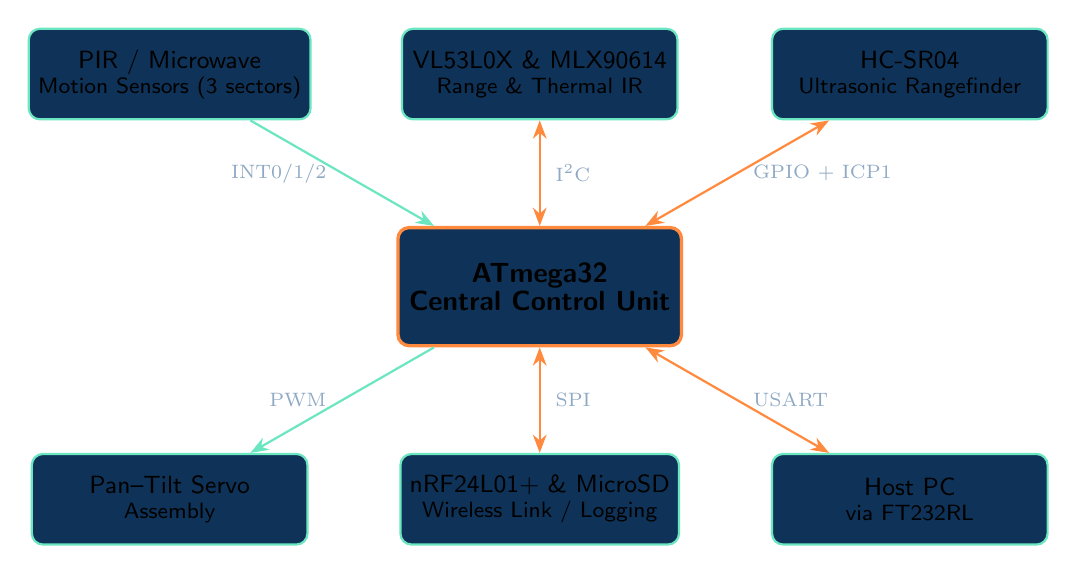
\begin{tikzpicture}[
            mcu/.style={rectangle, draw=AmberAccent, very thick, fill=CardBg, rounded corners, minimum height=1.5cm, minimum width=3.6cm, align=center, font=\sffamily\bfseries\normalsize},
            block/.style={rectangle, draw=TealAccent, thick, fill=CardBg, rounded corners, minimum height=1.15cm, minimum width=3.5cm, align=center, font=\sffamily\small},
            arrow/.style={-Stealth, thick, color=TealAccent},
            biarrow/.style={Stealth-Stealth, thick, color=AmberAccent},
            lbl/.style={font=\scriptsize, color=TextDim}
        ]
            % Sensing layer (top)
            \node[block] (pir) at (-4.7,2.7) {PIR / Microwave\\[-2pt]\footnotesize Motion Sensors (3 sectors)};
            \node[block] (optical) at (0,2.7) {VL53L0X \& MLX90614\\[-2pt]\footnotesize Range \& Thermal IR};
            \node[block] (ultra) at (4.7,2.7) {HC-SR04\\[-2pt]\footnotesize Ultrasonic Rangefinder};

            % Central controller
            \node[mcu] (mcu) at (0,0) {ATmega32\\[-2pt]\normalsize Central Control Unit};

            % Actuation / output layer (bottom)
            \node[block] (servo) at (-4.7,-2.7) {Pan--Tilt Servo\\[-2pt]\footnotesize Assembly};
            \node[block] (wireless) at (0,-2.7) {nRF24L01+ \& MicroSD\\[-2pt]\footnotesize Wireless Link / Logging};
            \node[block] (pc) at (4.7,-2.7) {Host PC\\[-2pt]\footnotesize via FT232RL};

            % Sensing arrows (into MCU)
            \draw[arrow] (pir) -- node[lbl, left, xshift=-2pt]{INT0/1/2} (mcu);
            \draw[biarrow] (optical) -- node[lbl, right, xshift=2pt]{I$^2$C} (mcu);
            \draw[biarrow] (ultra) -- node[lbl, right, xshift=2pt]{GPIO + ICP1} (mcu);

            % Output arrows (from MCU)
            \draw[arrow] (mcu) -- node[lbl, left, xshift=-2pt]{PWM} (servo);
            \draw[biarrow] (mcu) -- node[lbl, right, xshift=2pt]{SPI} (wireless);
            \draw[biarrow] (mcu) -- node[lbl, right, xshift=2pt]{USART} (pc);
        \end{tikzpicture}
    }
    \vspace{0.1cm}

    {\tiny \color{TextDim} $\rightarrow$ one-way signal \quad $\leftrightarrow$ shared bus \quad -- the ATmega32 is the single point of coordination for all sensing, actuation, and communication.}
\end{frame}

% --- SLIDE 6: SYSTEM DESIGN - COMPONENT ROLES & PINS ---
\begin{frame}{3. System Design: Component Roles \& Key Interfaces}
    \small
    \begin{table}
        \centering
        \color{TextInk}
        \begin{tabular}{llp{5.3cm}}
            \toprule
            \textbf{\color{AmberAccent} Component} & \textbf{\color{AmberAccent} Interface} & \textbf{\color{AmberAccent} Role \& ATmega32 Pin Mapping} \\
            \midrule
            PIR / Microwave Array & External INT & Coarse detection; \texttt{INT0 (PD2)}, \texttt{INT1 (PD3)}, \texttt{INT2 (PB2)} \\
            VL53L0X Laser ToF & I$^2$C (0x29) & Chest-height range check; shared TWI bus @ 100 kHz \\
            HC-SR04 Ultrasonic & GPIO + Timer1 & Ankle-height range check; \texttt{PA1} (Trig) / \texttt{PD6} (Echo via ICP1) \\
            MLX90614 Thermal IR & I$^2$C (0x5A) & Contactless body-heat check; shared TWI bus \\
            Pan / Tilt Servos & Hardware PWM & Sensor cluster orientation; Timer0 \texttt{OC0 (PB3)} / Timer2 \texttt{OC2 (PD7)} \\
            nRF24L01+ Transceiver & Hardware SPI & Wireless identification link; \texttt{PD5} (CS\_RF) \\
            MicroSD Module & Hardware SPI & Local event logging; \texttt{PD4} (CS\_SD) \\
            FT232RL USB Bridge & USART & Telemetry to host PC; 115200 baud (\texttt{RXD/TXD}) \\
            \bottomrule
        \end{tabular}
    \end{table}
\end{frame}

% --- SLIDE 7: SYSTEM DESIGN - OPERATIONAL LOGIC (FSM) ---
\begin{frame}{3. System Design: Operational Logic}
    \centering
    \resizebox{0.92\textwidth}{!}{
        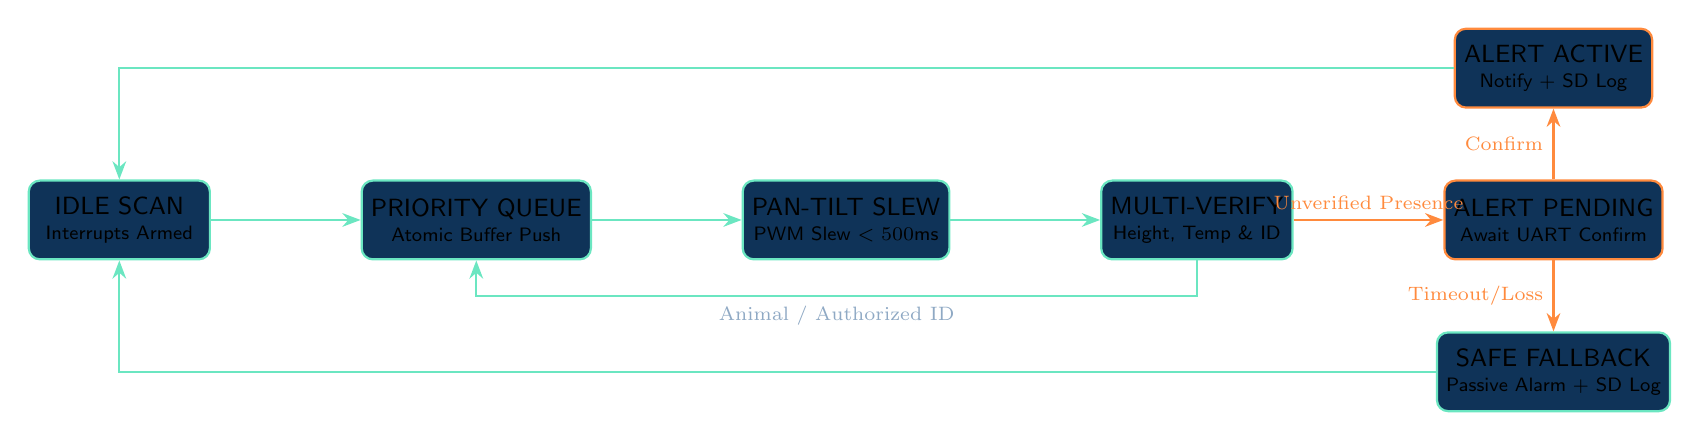
\begin{tikzpicture}[
            node distance=1.9cm,
            state/.style={rectangle, draw=TealAccent, fill=CardBg, thick, rounded corners, minimum height=1cm, minimum width=2.3cm, align=center, font=\sffamily\small},
            alertstate/.style={state, draw=AmberAccent, fill=CardBg},
            arrow/.style={-Stealth, thick, color=TealAccent},
            alertarrow/.style={-Stealth, thick, color=AmberAccent}
        ]
            \node[state] (idle) {IDLE SCAN\\[-2pt]\scriptsize Interrupts Armed};
            \node[state, right=of idle] (queue) {PRIORITY QUEUE\\[-2pt]\scriptsize Atomic Buffer Push};
            \node[state, right=of queue] (slew) {PAN-TILT SLEW\\[-2pt]\scriptsize PWM Slew $<500$ms};
            \node[state, right=of slew] (verify) {MULTI-VERIFY\\[-2pt]\scriptsize Height, Temp \& ID};
            \node[alertstate, right=of verify] (locked) {ALERT PENDING\\[-2pt]\scriptsize Await UART Confirm};
            \node[alertstate, above=0.9cm of locked] (fire) {ALERT ACTIVE\\[-2pt]\scriptsize Notify + SD Log};
            \node[state, below=0.9cm of locked] (fallback) {SAFE FALLBACK\\[-2pt]\scriptsize Passive Alarm + SD Log};

            \draw[arrow] (idle) -- (queue);
            \draw[arrow] (queue) -- (slew);
            \draw[arrow] (slew) -- (verify);
            \draw[alertarrow] (verify) -- node[above, font=\scriptsize, color=AmberAccent]{Unverified Presence} (locked);
            \draw[alertarrow] (locked) -- node[left, font=\scriptsize, color=AmberAccent]{Confirm} (fire);
            \draw[alertarrow] (locked) -- node[left, font=\scriptsize, color=AmberAccent]{Timeout/Loss} (fallback);
            \draw[arrow] (verify.south) -- ++(0,-0.45) -| node[near start, below, font=\scriptsize, color=TextDim]{Animal / Authorized ID} (queue.south);
            \draw[arrow] (fire.west) -| (idle.north);
            \draw[arrow] (fallback.west) -| (idle.south);
        \end{tikzpicture}
    }
    \vspace{0.25cm}
    \begin{itemize}
        \small
        \item Non-target detections auto-dismiss back to the queue/idle state without operator disruption.
        \item \textbf{\color{TealAccent}Teal} states are normal operation; \textbf{\color{AmberAccent}amber} states involve an alert decision or its outcome.
    \end{itemize}
\end{frame}

% --- SLIDE 8: ROLE OF THE ATMEGA32 ---
\begin{frame}{4. Role of the ATmega32}
    \begin{columns}[T]
        \begin{column}{0.48\textwidth}
            \begin{block}{Tasks Performed}
                \small
                \begin{itemize}
                    \item Runs the full state-machine control logic: idle scan, queuing, slewing, verification, alerting.
                    \item Reads and fuses data from five independent sensor sources in real time.
                    \item Drives closed-loop pan-tilt actuation.
                    \item Arbitrates two shared buses (I$^2$C and SPI) between multiple peripherals.
                    \item Streams telemetry and parses operator commands over UART.
                \end{itemize}
            \end{block}
        \end{column}
        \begin{column}{0.48\textwidth}
            \begin{block}{Peripheral Features Used}
                \small
                \begin{itemize}
                    \item \textbf{GPIO} -- trigger line, chip-select lines
                    \item \textbf{Ext. Interrupts} -- INT0--INT2 motion capture
                    \item \textbf{Timers / PWM} -- Timer0/2 for servos; Timer1 for scheduling \& ICP1 echo capture
                    \item \textbf{USART} -- 115200 baud telemetry \& commands
                    \item \textbf{SPI} -- nRF24L01+ and MicroSD, multiplexed
                    \item \textbf{I$^2$C (TWI)} -- VL53L0X and MLX90614
                \end{itemize}
            \end{block}
        \end{column}
    \end{columns}
    \vspace{0.15cm}
    \footnotesize\color{TextDim} On-chip ADC is not required by the current sensor set; the pin is reserved for a future analog sensor addition (Section 8).
\end{frame}

% --- SLIDE 9: IMPLEMENTATION PLAN - MILESTONES ---
\begin{frame}{5. Implementation Plan: Milestones}
    \small \textbf{Expected outcome:} a prototype that autonomously detects, localizes, and verifies a perimeter event, then requests operator confirmation before alerting -- with events logged locally and visible on a host-side monitor.
    \vspace{0.2cm}
    \begin{columns}[T]
        \begin{column}{0.48\textwidth}
            \begin{block}{Stage 1 -- Project Update 1 (Wks 1--3)}
                \footnotesize
                \begin{itemize}
                    \item MCU bring-up, PWM calibration, I$^2$C drivers, non-blocking ICP1 echo timing.
                    \item Multi-sector interrupts and ISR priority queue.
                    \item \textbf{Dependency:} sensor drivers and PWM calibration validated before slewing tests.
                    \item \textbf{Milestone:} slewing, dual-beam classification, telemetry working end-to-end.
                \end{itemize}
            \end{block}
        \end{column}
        \begin{column}{0.48\textwidth}
            \begin{block}{Stage 2 -- Final Submission (Wks 4--6)}
                \footnotesize
                \begin{itemize}
                    \item SPI multiplexing, wireless ID handshake, monitoring GUI, UART safety interlock.
                    \item \textbf{Dependency:} handshake needs a stable shared SPI bus; GUI needs a finalized telemetry format.
                    \item \textbf{Milestone:} autonomous prototype with operator-gated alerting, validated in field testing.
                \end{itemize}
            \end{block}
        \end{column}
    \end{columns}
\end{frame}

% --- SLIDE 10: IMPLEMENTATION PLAN - TEAM RESPONSIBILITIES ---
\begin{frame}{5. Implementation Plan: Team Responsibilities}
    \begin{columns}[T]
        \begin{column}{0.32\textwidth}
            \begin{block}{Member 1: Firmware \& Control}
                \small
                \begin{itemize}
                    \item Bare-metal AVR C drivers
                    \item Core FSM architecture
                    \item ISR priority queue
                    \item Servo PWM \& timing loops
                \end{itemize}
            \end{block}
        \end{column}
        \begin{column}{0.32\textwidth}
            \begin{block}{Member 2: Hardware \& Power}
                \small
                \begin{itemize}
                    \item Pan-tilt mechanical build
                    \item LM2596 power rails
                    \item Motor driver stage
                    \item EMI \& power decoupling
                \end{itemize}
            \end{block}
        \end{column}
        \begin{column}{0.32\textwidth}
            \begin{block}{Member 3: Systems \& GUI}
                \small
                \begin{itemize}
                    \item SPI bus multiplexing
                    \item nRF24L01+ handshake
                    \item MicroSD FAT logging
                    \item Python monitoring GUI
                \end{itemize}
            \end{block}
        \end{column}
    \end{columns}
\end{frame}

% --- SLIDE 11: USE OF OTHER CONTROLLERS (OPTIONAL) ---
\begin{frame}{6. Use of Other Controllers (Optional)}
    \begin{block}{Current Design}
        \small The core system is fully self-contained on the ATmega32; no secondary microcontroller is required for the planned scope of this project.
    \end{block}
    \begin{block}{Potential Future Use}
        \small If visual classification is added as a future extension (Section 8), an ESP32-CAM co-processor could handle image capture and inference, sending results to the ATmega32 over UART or SPI as a simple event flag. This is not part of the current 6-week implementation plan.
    \end{block}
\end{frame}

% --- SLIDE 12: TESTING AND SUCCESS CRITERIA ---
\begin{frame}{7. Testing \& Success Criteria}
    \scriptsize
    \begin{table}
        \centering
        \color{TextInk}
        \begin{tabular}{llll}
            \toprule
            \textbf{\color{AmberAccent} Metric} & \textbf{\color{AmberAccent} Target} & \textbf{\color{AmberAccent} Test Method} & \textbf{\color{AmberAccent} Priority} \\
            \midrule
            Turret slew speed & $< 500$ ms & Oscilloscope PWM step response & Essential \\
            Distance accuracy & $\pm 5$ mm at $\le 1.5$ m & Bench test vs.\ VL53L0X & Essential \\
            Classification accuracy & $\ge 90\%$ & Multi-trial human vs.\ animal tests & Essential \\
            Queue integrity & 100\% capture, 0 dropped & Simultaneous 3-sector stress test & Essential \\
            Safety interlock & 0 unconfirmed alerts & Link-severing / timeout test & Essential \\
            Thermal resolution & $\Delta T \ge 3^\circ\text{C}$ & Controlled heat-source pass test & Optional \\
            ID handshake speed & $< 30$ ms & Logic analyzer timing (SPI) & Optional \\
            Monitoring GUI & Live 10 Hz update & Manual end-to-end review & Optional \\
            \bottomrule
        \end{tabular}
    \end{table}
    \vspace{0.2cm}
    \footnotesize Essential criteria define a working core system (detection, verification, safe alerting); optional criteria are stretch goals that are not required for project success.
\end{frame}

% --- SLIDE 13: CHALLENGES AND FUTURE SCOPE ---
\begin{frame}{8. Challenges \& Future Scope}
    \begin{columns}[T]
        \begin{column}{0.48\textwidth}
            \begin{block}{Anticipated Challenges}
                \footnotesize
                \begin{itemize}
                    \item \textbf{SPI contention:} explicit bus-release routines and dedicated chip-select lines.
                    \item \textbf{Servo electrical noise:} isolated LM2596 rails with bulk decoupling.
                    \item \textbf{Timer1 dual use:} ICP1 reads \texttt{TCNT1} without resetting the counter.
                    \item \textbf{I$^2$C arbitration:} bus timeout and retry logic for differing clock-stretch.
                    \item \textbf{Memory limits:} 2 KB SRAM / 32 KB Flash require lightweight, fixed-size C buffers rather than dynamic allocation.
                \end{itemize}
            \end{block}
        \end{column}
        \begin{column}{0.48\textwidth}
            \begin{block}{Future Scope \& Scalability}
                \footnotesize
                \begin{itemize}
                    \item \textbf{Multi-node mesh:} existing nRF24L01+ radios link units for wider coverage.
                    \item \textbf{Central dashboard:} a gateway aggregates telemetry from multiple nodes.
                    \item \textbf{Vision upgrade:} AMG8833 thermal array or ESP32-CAM co-processor.
                    \item \textbf{Full coverage:} slip-ring and stepper motor for continuous $360^\circ$ tracking.
                    \item \textbf{Off-grid power:} solar charging and battery management.
                    \item \textbf{Platform migration:} move to a 32-bit MCU if features need more headroom.
                \end{itemize}
            \end{block}
        \end{column}
    \end{columns}
\end{frame}

\end{document}
